\documentclass[12pt,a4paper,oneside]{report}
\usepackage[a4paper,left=4cm,right=3cm,top=3cm,bottom=3cm]{geometry}
\usepackage[utf8]{inputenc}
\usepackage{ucs}
\usepackage{amsmath}
\usepackage{amsfonts}
\usepackage{amssymb}
\usepackage{makeidx}
\usepackage{graphicx}
\usepackage{anyfontsize}
\usepackage{setspace}
\usepackage{booktabs}
\usepackage{multirow}
\usepackage[table,xcdraw]{xcolor}
\usepackage{url}
\usepackage[bahasa]{babel}
\usepackage{graphicx}
\usepackage{color,soul}
\usepackage{titlesec}
\usepackage{lipsum}
\usepackage[subpreambles=true]{standalone}
\usepackage{subfiles}
\usepackage{pdfpages}

\graphicspath{{images/}}

\titleformat{\chapter}[block]
{\centering\fontsize{16}{1}\huge\bfseries}{Bab \thechapter.}{0.1em}{\Huge}

\titleformat{\section}[block]
{\fontsize{14}{1}\bfseries}{\thesection.}{0.1em}{}

\addto{\captionsbahasa}{\renewcommand{\abstractname}{Abstrak}}
\addto{\captionsbahasa}{\renewcommand{\bibname}{Daftar Pustaka}}

\providecommand{\katakunci}[1]{\textbf{\textit{Kata kunci:}} #1}
\providecommand{\katakunciENG}[1]{\textbf{\textit{Keyword(s):}} #1}
\providecommand{\keywords}[1]{\textbf{\textit{Keywords:}} #1}
\providecommand{\judulta}{\textbf{Implementasi Algoritma \textit{Merging Context Seeds} untuk \textit{Plagiarism Detection}}}
\providecommand{\tglefektif}{Bandung, 29 Maret 2016}

\newcommand{\source}[1]{\caption*{Sumber: {#1}} }
\newcommand{\doublesignature}[6]{
	\parbox{\linewidth}{
		\parbox{0.48\linewidth}{
			\centering
			#1
		}
		\hfill
		\parbox{0.48\linewidth}{
			\centering
			#2
		}
	}\\[3cm]
	\parbox{\linewidth}{
		\parbox{0.48\linewidth}{
			\centering
			\rule{0.5\linewidth}{1pt}\\
			#3\\
			#4 
		}
		\hfill
		\parbox{0.48\linewidth}{
			\centering
			\rule{0.5\linewidth}{1pt}\\
			#5\\
			#6
		}
	}
}

\begin{document}
	
	%Cover
	\subfile{_other/Cover}	
	
	
	\pagenumbering{roman}
	\setcounter{page}{1}	
	%Lembar Persetujuan
	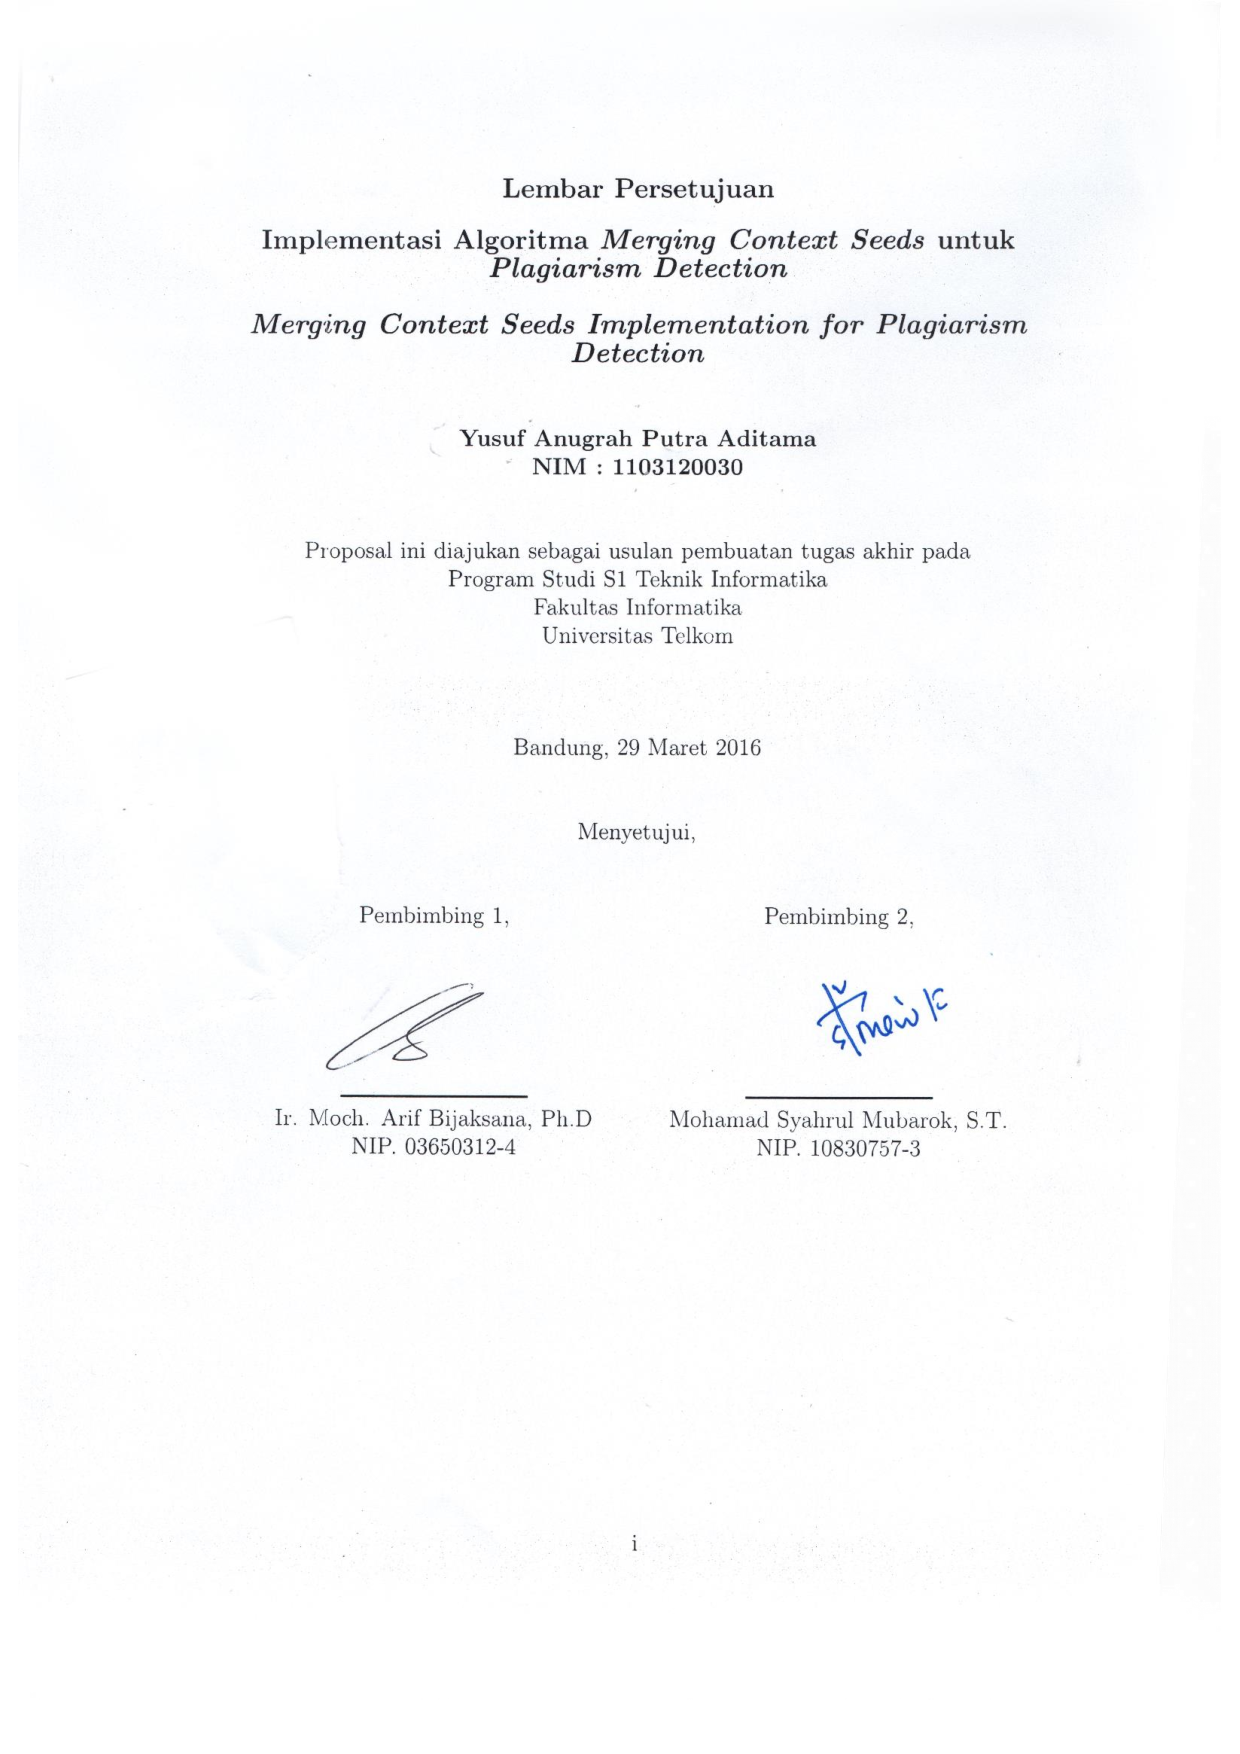
\includepdf{_other/Pengesahan_TTD.pdf} %nyalakan ini
	%\subfile{_other/Lembar_Persetujuan} %atau ini
	
	
	%Daftar Isi
	\tableofcontents
	\newpage
	
	
	%Abstrak
	\subfile{_other/Abstrak}
	\newpage
	\subfile{_other/Abstract}
	
	
	\setcounter{page}{1}
	\pagenumbering{arabic}
	
	%Bab-1
	\chapter{Pendahuluan}
	\subfile{_bab1/Latar_Belakang}
	\subfile{_bab1/Rumusan_Masalah}
	\subfile{_bab1/Tujuan}
	\subfile{_bab1/Batasan_Masalah}
	\subfile{_bab1/Hipotesa}
	\subfile{_bab1/Metedeologi}
	\subfile{_bab1/Jadwal_Kegiatan}
	
	%Bab-2
	\chapter{Tinjauan Pustaka}
	\subfile{_bab2/Plagiarism}
	\subfile{_bab2/Plagiarism_Detection}
	\subfile{_bab2/NGram}
	\subfile{_bab2/Merging_Context_Seed}
	\subfile{_bab2/KNN}
	\subfile{_bab2/FMeasure}
	\subfile{_bab2/Dataset}
	
	%Bab-3
	\chapter{Metodologi dan Desain Sistem}
	\subfile{_bab3/Analisis_Kebutuhan}
	\subfile{_bab3/Perancangan_Sistem}
	\subfile{_bab3/Pengujian}
	
	%Daftar Pustaka
	\bibliographystyle{IEEEtran}
	\bibliography{references-proposal-ta}
	
	
\end{document}